\apendice{Estudio experimental}
John Brooke describe en 1996 una escala de usabilidad barata que puede ser utilizada para la evaluación global de la usabilidad de sistemas: la escala SUS (System Usability Scale) \cite{inbook}. Se trata de una escala Likert con 10 puntos claves para que indivíduos que hayan probado el sistema evalúen la usabilidad general del mismo.

Los indivíduos responden con una cifra del 1 al 5 (1 expresando completo desacuerdo y 5 expresando completo acuerdo) a 10 afirmaciones:
\begin{enumerate}
    \item Me gustaría utilizar el sistema de forma frecuente
    \item El sistema me parece innecesariamente complejo
    \item Creo que el sistema es fácil de utilizar
    \item Creo que necesitaría apoyo de personal técnico para poder utilizar el sistema
    \item Encuentro las diferentes funciones del sistema bien integradas
    \item Creo que hay demasiadas incosistencias en el sistema
    \item Imagino que la mayoría de gente aprendería a utilizar el sistema muy rápidamente
    \item Encuentro la utilización del sistema muy incómoda
    \item Me sentí muy confiado utilizando el sistema
    \item Necesité aprender muchas cosas antes de poder utilizar el sistema
\end{enumerate}
\section{Detalle de resultados.}
Con el objetivo de evaluar la usabilidad de la solución tecnológica propuesta para pacientes con Párkinson y profesionales, se realizó una demostración del funcionamiento del software y hardware en la Asociación de Párkinson de Burgos. Posteriormente, se envió a los profesionales de dicha asociación que habían presenciado la demostración una encuesta SUS (System Usability Scale) realizada mediante Google Forms para obtener un primer feedback proveniente de personal especializado.

La encuesta fue rellenada por un profesional de la salud de la asociación, obteniendo los siguientes resultados\ref{fig:encuesta1} \ref{fig:encuesta2} \ref{fig:encuesta3}:
    \begin{figure}[h]
        \centering
        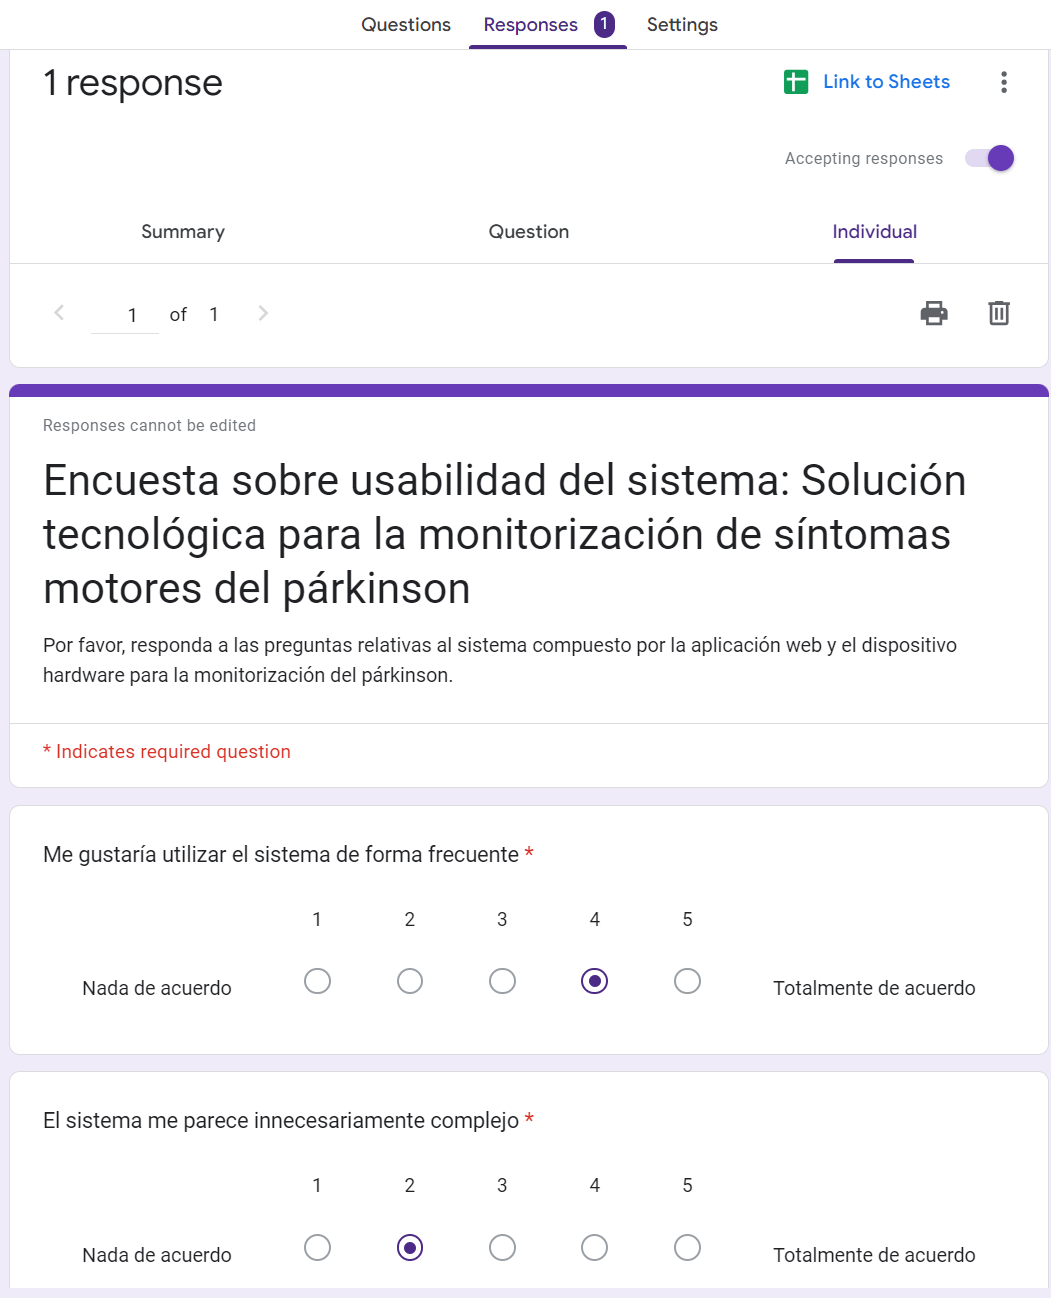
\includegraphics[width=1\textwidth]{img/encuesta1.png}
        \caption{Resultados de la encuesta SUS, parte 1. Fuente propia.}
        \label{fig:encuesta1}
    \end{figure}
        \begin{figure}[h]
        \centering
        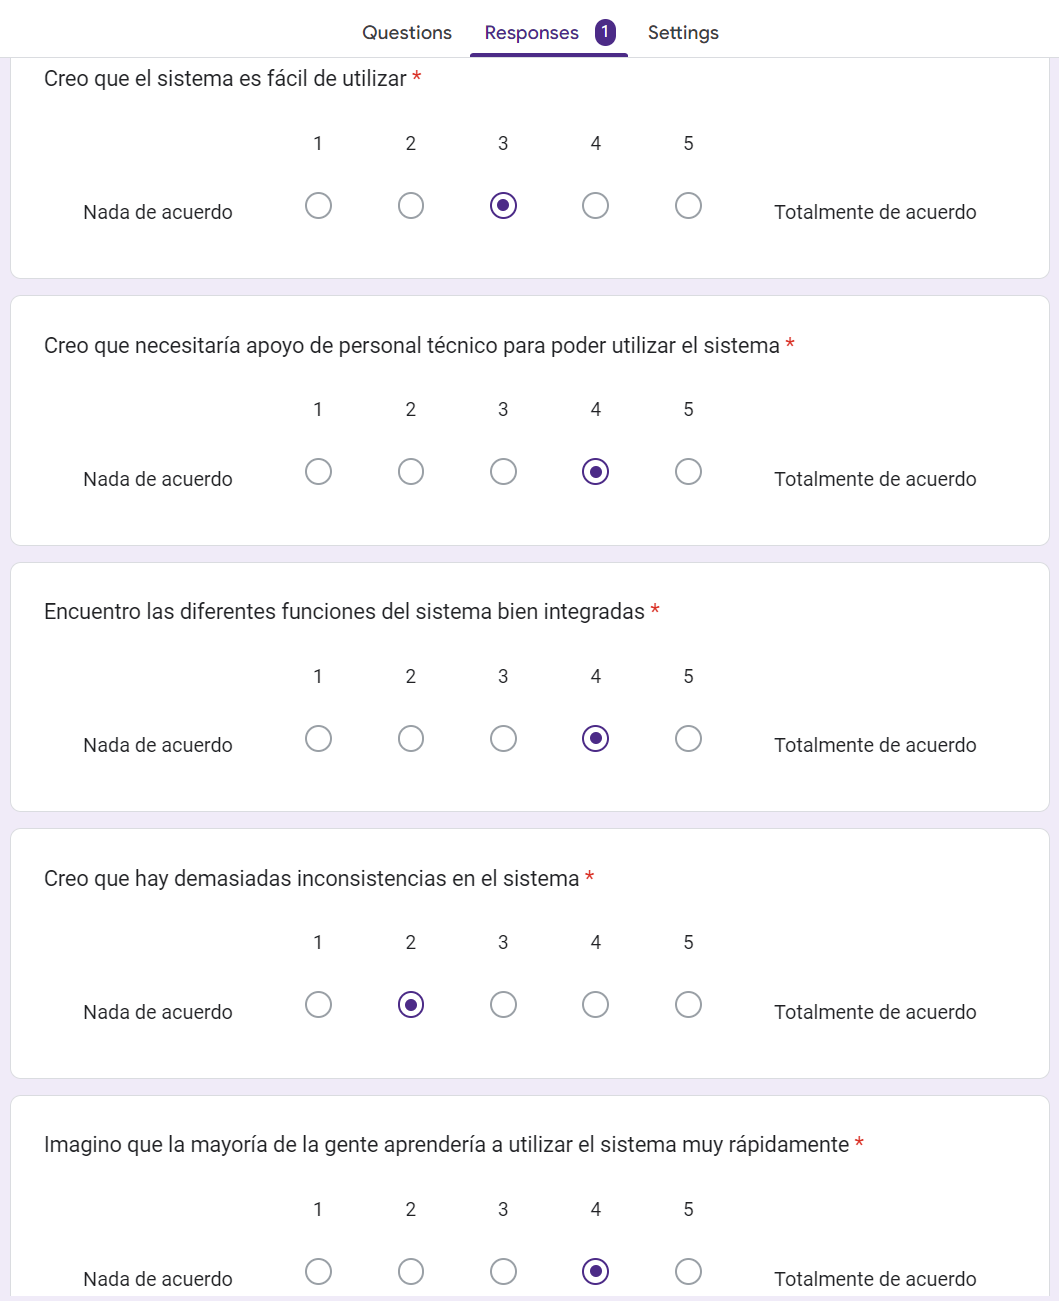
\includegraphics[width=1\textwidth]{img/encuesta2.png}
        \caption{Resultados de la encuesta SUS, parte 2. Fuente propia.}
        \label{fig:encuesta2}
    \end{figure}
        \begin{figure}[h]
        \centering
        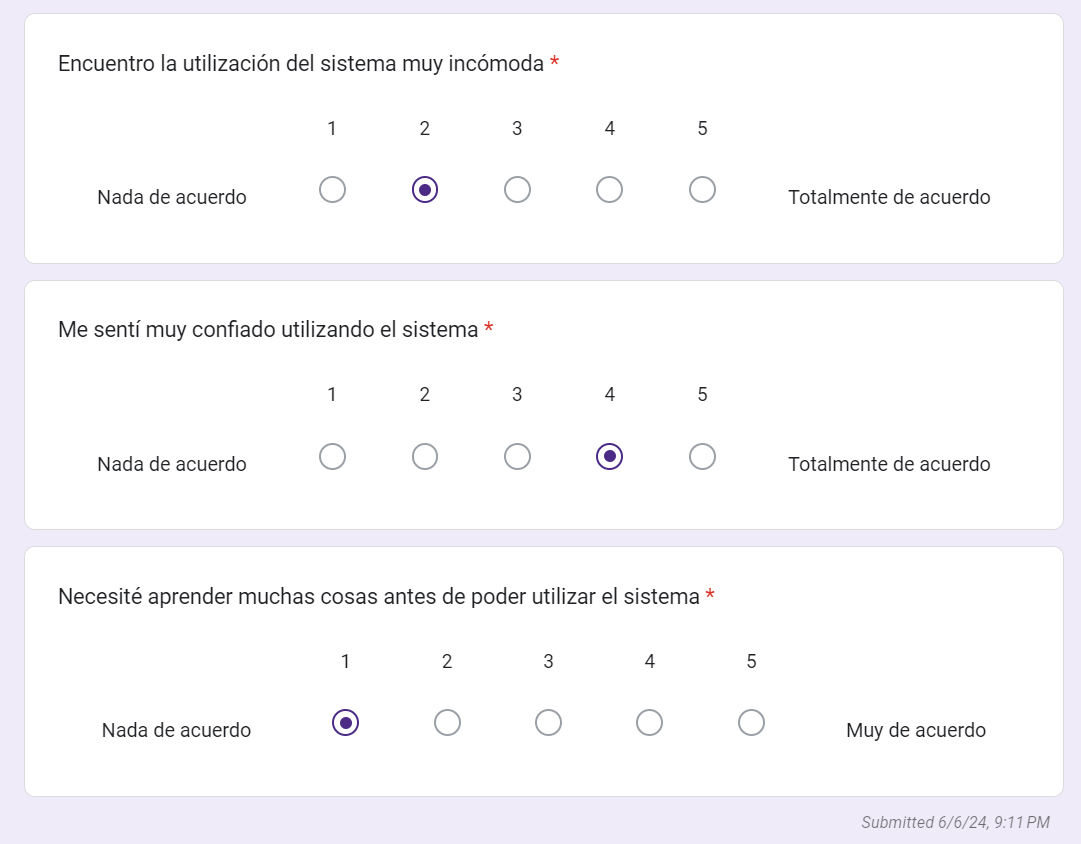
\includegraphics[width=1\textwidth]{img/encuesta3.png}
        \caption{Resultados de la encuesta SUS, parte 3. Fuente propia.}
        \label{fig:encuesta3}
    \end{figure}
Tal y como observamos en el artículo \cite{kaya2019usability}, el cálculo del 'score' o puntuación de una encuesta SUS se realiza de la siguiente forma:
\begin{enumerate}
    \item La puntuación correspondiente a las respuestas a preguntas impares (positivas), se calculan restando 1 al resultado obtenido. En este caso los resultados de la encuesta son 4, 3, 4, 4 y 4; por lo cual obtendríamos los números 3,2,3,3 y 3. La suma de estas puntuaciones es 14.
    \item La puntuación correspondiente a las respuestas a preguntas pares (negativas), se calcula restando al número 5 el resultado obtenido, es decir, con los resultados de la encuesta 2,4,2,2 y 1 obtendríamos los números 3,1,3,3 y 4. La suma de estas puntuaciones es 14.
    \item Para obtener la puntuación final (del 0 al 100), multiplicaremos por 2.5 la suma de ambas puntuaciones, es decir (14+14)*2.5 = 70.
\end{enumerate}
En el artículo \cite{sauro2016quantifying}, se establece 68 como puntuación media en encuestas SUS, teniendo una desviación estandar de 12.5. Como podemos observar en la tabla \ref{fig:sus}, la puntuación obtenida (70 puntos), se sitúa por encima del 56 por ciento de los sistemas analizados con esta escala. Esto refleja una relativa aceptabilidad del sistema, presentando también un ámplio rango de mejora en la facilidad de uso del mismo. En particular, el enunciado en el cual se obtuvo una respuesta más negativa fue 'Creo que necesitaría apoyo de personal técnico para poder utilizar el sistema'.

Es necesario tener en cuenta que estos resultados tienen una validez limitada, debido a que se obtuvieron a partir de las respuestas de un sólo participante. Sin embargo, teniendo en cuenta la similar reacción de todos los profesionales de la asociación de Párkinson que presenciaron la demostración y que el presente producto es tan sólo un prototipo, esta evaluación es suficiente para obtener una primera idea sobre qué puntos deberían mejorarse en futuras versiones del prototipo.
        \begin{figure}[h]
        \centering
        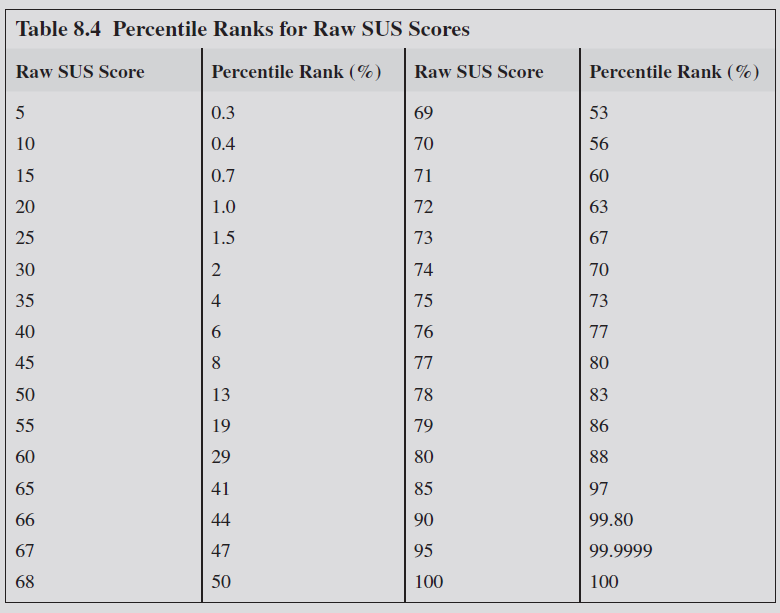
\includegraphics[width=1\textwidth]{img/sus.png}
        \caption{Tabla relacionando puntuaciones SUS con el rango de percentils percentiles \cite{sauro2016quantifying}.}
        \label{fig:sus}
    \end{figure}